
\documentclass[./EngineeringMaths.tex]{subfiles}

\begin{document}
\section[Set Theory]{Set Theory}
A Set is a collection of well defined objects which is denoted by a capital letter and it's elements are described by small letters or numbers.

% = = = = = = TYPES OF SET = = = = = =
\subsection*{Types of Sets}
\begin{itemize}
\item Universal Set ($\xi$ or $U$)
\item Null Set ($\phi$)
\item Subset ($\subset$)
\item Superset ($\supset$)
\item Compliment of a set ($A^c$ or $\bar{A}$)
\item Equal Sets ($=$)
\end{itemize}

% = = = = = = OPERATIONS ON SETS = = = = = =
\subsection*{Operations on Sets}
\begin{itemize}
\item Union ($\cap$)
\item Intersection ($\cup$)
\item De Morgans
\item Laws - Associative, Distributive
\end{itemize}

% = = = = = = TERMINOLOGY = = = = = =
\subsection{Random Experiments, Events and more}
If the repetition of an experiment under identical condition results in different possible outcomes, then such an experiment is called Randome Experiment or Stochastic Experiment.

\textbf{Sample Space (\textbf{S})} is a set of all possible outcomes of a random experiment.\

\textbf{Event ($\mathbf{E}$)} is a subset of Sample Space \textbf{S}

\fbox{Example} Tossing of coin: \textbf{S} = \{H,T\}

\subsection*{Types of Events}

\begin{itemize}
\item Mutually Exclusive
\item Equally Likely
\end{itemize}

% = = = = = = PROBABILITY = = = = = =
\subsection{Probability}

Let \textbf{A} be an event of \textbf{S}. If \textbf{A} occurs $m$ different ways out of a total of $n$, then probability of \textbf{A} is denoted by 

\begin{center}
    $P(A) = \frac{Favorable\ Cases}{Total\ Outcomes} = \frac{m}{n}$
\end{center}

% - - - - - - AXIOMS - - - - - -
\subsubsection[Axioms on Probability]{Kalmogorov's Axioms}

Let \textbf{E} be an experiment with sample space \textbf{S}.
Let \textbf{A} be an event of \textbf{S}, then:

\begin{itemize}
\item $0 \leq P(A) \leq 1$ \label{th:1}
\item $P(S) = 1$ \label{th:2}
\item Given A \& B are mutually exclusive then, $P(A\cup B) = P(A) + P(B)$ \label{th:3}
\item If $A_1,A_2,A_3...A_n$ are mutually exclusive then, $P(\cup_{i=1}^n A_i) = \sum_{i=1}^n P(A_i)$ \label{th:4}
\end{itemize}

% + + + + + + THEOREM + + + + + +
\begin{theorem}
If A is an event of S then,

\begin{enumerate}[i]
\item $P(\phi) = 0$
\item $P(A)+P(\bar{A})=1$
\end{enumerate}
\end{theorem}
\begin{proof}
i) Let $A\cup \phi = \phi$
\begin{subequations}
\begin{equation}
A\cap \phi = \phi
\end{equation}
\[ P(A\cap \phi) = P(\phi) \]
\begin{equation}
A\cup \phi = \phi \label{eq:1}
\end{equation}
\[ P(A\cup \phi) = P(\phi) \]

Using axiom from \ref{th:3} \& equation.\eqref{eq:1} we get,

\[ P(A) + P(\phi) = P(A) \]
\[ P(\phi) = 0 \]
\end{subequations}

\begin{subequations}
ii) Let $S = A \cup \bar{A}$
\begin{equation*}
P(S) = P(A \cup \bar{A}) \tag*{[Mutually Exclusive]} \\
\end{equation*}
\[ 1 = P(A) + P(\bar{A}) \]
\[ P(A) + P(\bar{A}) = 1 \]
\end{subequations}
\end{proof}

% - - - - - - ADDITION RULE - - - - - -
\subsubsection{Addition Rule}
If A \& B are two events then $P(A\cup B)=P(A)+P(B)-P(A\cap B)$ by addition rule.

\begin{proof}
\begin{subequations}
Consider the following venn diagram having sets A and B.

\begin{center}
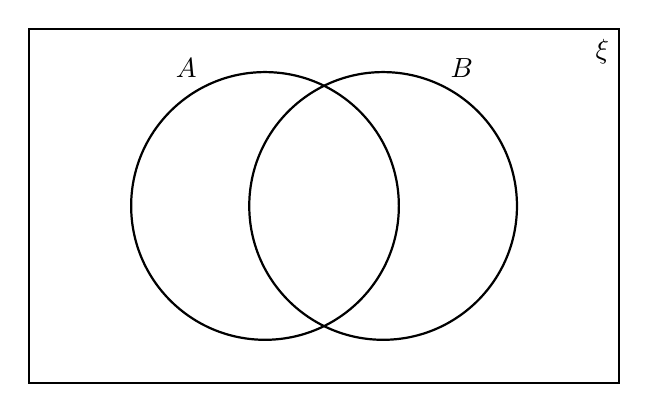
\begin{tikzpicture}[thick]
\draw (0,0) rectangle (7.5,4.5) node[anchor=north east] {$\xi$};
\draw (3,2.25) circle (1.7cm) node[above,shift={(-1,1.5)}] {$A$};
\draw (4.5,2.25) circle (1.7cm) node[above,shift={(1,1.5)}] {$B$};
\end{tikzpicture}
\end{center}
\[A\cup B = (A\cap \bar{B})\cup(A\cap B)\cup(\bar{A}\cap B)\]

Consider,\quad \quad \(B = (A\cap B)\cup(\bar{A}\cap B)\)
\[P(B) = P((A\cap B)\cup(\bar{A}\cap B)) \tag*{[Mutually Exclusive]}\]
\begin{equation}
P(B) = P(A\cap B)\cup P(\bar{A}\cap B) \label{eq:2}
\end{equation}

Consider,\quad \quad \(A = (A\cap B)\cup(A\cap \bar{B})\)
\[P(B) = P((A\cap B)\cup(A\cap \bar{B})) \tag*{[Mutually Exclusive]}\]
\begin{equation}
P(B) = P(A\cap B)\cup P(A\cap \bar{B}) \label{eq:3}
\end{equation}

Thus from \eqref{eq:2} and \eqref{eq:3} we get,
\begin{center}
\fbox{\(P(A\cup B)=P(A)+P(B)-P(A\cap B)\)}
\end{center}
\end{subequations}
\end{proof}

\end{document}